\documentclass[a4paper,11pt,oneside]{book}

\newcommand{\standalone}{}
%%% το αρχείο αυτό καθορίζει το look που έχουν οι pythonies
%%% γίνεται \input από όλα τα κεφάλαια και τα φύλλα εργασίας

% χρησιμοποιούμενα πακέτα: 
% 
% polyglossia
% xstring
% graphicx
% caption
% xcolor
% hyperref
% minted
% geometry
% titlesec
% datetime
% changepage
% ntheorem

% οριζόμενες εντολές:
%
% smallcaps (βοηθ. removeaccents)
%    μικρά κεφαλαία χωρίς τόνους στα φωνήεντα
% scaling
%    η κλιμάκωση *όλων* των illustrations, τρέχουσα τιμή 0.9
% iconcomputer, iconkeyboard, icondiscuss, iconfillin, iconcaution, iconprompt, dottedline
%    εικονίδια για τα φύλλα εργασίας και εστιγμένη γραμμή
% marginnote
%    πλευρικό σχόλιο
% chapterwabstract (βοηθ. abstract, boxcolor, chaptercolor, concepts, tmpconcepts)
%    εισαγωγικό κείμενο κεφαλαίου με χρωματιστό τετράγωνο, συνοδευτικές έννοιες, κλπ.
% tobecontinued
%    εμφανίζει το "συνεχίζεται στην επόμενη σελίδα"

% οριζόμενα περιβάλλοντα:
% 
% note
%    μια υποσημείωση ή υπόδειξη, με μικρότερα γράμματα
% question
%    μια ερώτηση που "οδηγεί" κάθε νέα ενότητα
% answer
%    μια απάντηση σε μια ερώτηση του φύλλου εργασίας
% theory
%    μια ενότητα "θεωρίας" (στο τέλος ενός κεφαλαίου)
% exercise
%    μια αριθμημένη άσκηση
% step
%    ένα αριθμημένο βήμα (για φύλλο εργασίας)

% για μορφοποίηση κώδικα:
%
% pycode (περιβάλλον)
%     κώδικας python χωρίς αρίθμηση
% pyfile (εντολή)
%     εισαγωγή κώδικα python από αρχείο
% pyfilenl (εντολή)
%     εισαγωγή κώδικα python από αρχείο χωρίς αρίθμηση γραμμών
% pyfilesrc (εντολή)
%    εισαγωγή κώδικα από αρχείο με link στο αρχείο
% pyinline (εντολή)
%     κώδικας python μέσα στη ροή του κειμένου
% pyplain (περιβάλλον, για τα φύλλα εργασίας)
%     κώδικας python χωρίς φόντο
% pynew (περιβάλλον, για τα φύλλα εργασίας)
%     κώδικας python με φόντο
% pyterm (περιβάλλον για τα φύλλα εργασίας)
%     η είσοδος του χρήστη ή τα περιεχόμενα της οθόνης
% pyhighlight (εντολή)
%    highlight κειμένου (χρησιμοποιείται για κώδικα μέσα σε pyplain)


%%% επιλογές γλώσσας και γραμματοσειρών για το XeLaTeX

\usepackage{polyglossia}
\setdefaultlanguage{greek}
\setmainfont[Ligatures=TeX,SmallCapsFont={Linux Libertine O C},SmallCapsFeatures={Letters=SmallCaps}]{Linux Libertine O}
\setsansfont{Linux Biolinum O}
\setmonofont{Ubuntu Mono}
\enablehyphenation

% αφαίρεση τόνων από τα smallcaps
\usepackage{xstring}
\newcommand{\removeaccents}[1]{%
\def\result{#1}%
\StrSubstitute{\result}{ά}{α}[\result]%
\StrSubstitute{\result}{έ}{ε}[\result]%
\StrSubstitute{\result}{ή}{η}[\result]%
\StrSubstitute{\result}{ί}{ι}[\result]%
\StrSubstitute{\result}{ό}{ο}[\result]%
\StrSubstitute{\result}{ύ}{υ}[\result]%
\StrSubstitute{\result}{ώ}{ω}[\result]%
\StrSubstitute{\result}{Ά}{Α}[\result]%
\StrSubstitute{\result}{Έ}{Ε}[\result]%
\StrSubstitute{\result}{Ή}{Η}[\result]%
\StrSubstitute{\result}{Ί}{Ι}[\result]%
\StrSubstitute{\result}{Ό}{Ο}[\result]%
\StrSubstitute{\result}{Ύ}{Υ}[\result]%
\StrSubstitute{\result}{Ώ}{Ω}[\result]%
\result
}

\newcommand{\smallcaps}[1]{\textsc{\removeaccents{#1}}}

%%% εικόνες και λεζάντες

\usepackage{graphicx}
\newcommand{\scaling}{0.9}
\usepackage{caption}
\captionsetup{font=footnotesize}

%%% ειδικά περιβάλλοντα

\usepackage{xcolor}

% ερωτήσεις (που οδηγούν στην επόμενη ενότητα)
\definecolor{questioncolor}{rgb}{0.6,0.5,0.5}
\newenvironment{question}{\noindent\itshape\color{questioncolor}}{\noindent\ignorespaces}

% απαντήσεις (για τις ερωτήσεις των φύλλων εργασίας)
\definecolor{answercolor}{rgb}{0.5,0.5,0.5}
\newenvironment{answer}{\marginnote[16pt]{\iconfillin}\noindent\itshape\color{answercolor}}{\noindent\ignorespaces}

% περιβάλλον "θεωρίας" (πλήρες πλάτος κειμένου)
\usepackage{changepage}
\newenvironment{theory}[1]{\begin{adjustwidth}{}{-\overhang}\smallcaps{#1}\itshape}{\end{adjustwidth}}

% απομεινάρια...
% \newlength{\theoryrulelength}
% \setlength{\theoryrulelength}{36pt}
% \newenvironment{theory}{\rule{\theoryrulelength}{0.4pt}\begin{adjustwidth}{}{-\overhang}\itshape}{\end{adjustwidth}\rule{\theoryrulelength}{0.4pt}}

%%% υπερσύνδεσμοι

\definecolor{linkcolor}{rgb}{0.0,0.5,0.25}
\usepackage[colorlinks=true,urlcolor=linkcolor]{hyperref}

%%% εικονίδια και εστιγμένες γραμμές (για τα φύλλα εργασίας)

\newcommand{\iconcomputer}{
\includegraphics[scale=0.35]{../../share/circle-icons/one-color/computer.eps}}
\newcommand{\iconkeyboard}{
\includegraphics[scale=0.35]{../../share/circle-icons/one-color/keyboard.eps}}
\newcommand{\icondiscuss}{
\includegraphics[scale=0.35]{../../share/circle-icons/one-color/chat.eps}}
\newcommand{\iconfillin}{
\includegraphics[scale=0.35]{../../share/circle-icons/one-color/compose.eps}}
\newcommand{\iconcaution}{
\includegraphics[scale=0.35]{../../share/circle-icons/one-color/caution.eps}}
\newcommand{\iconprompt}{
\includegraphics[scale=0.35]{../../share/circle-icons/one-color/prompt.eps}}
\newcommand{\dottedline}{\vspace{\parskip}\dotfill}

%%% συνεχίζεται στην επόμενη σελίδα

\newcommand{\tobecontinued}{\mbox{}\hfill{\footnotesize ...συνεχίζεται στην επόμενη σελίδα.}}
\newenvironment{note}{\small\upshape}{}

%%% μορφοποίηση κώδικα με το pygmentize

\usepackage{minted}

% fix για ένα bug στο minted που εμφανίζεται όταν χρησιμοποιείται χρώμα στο φόντο (bgcolor)
% http://tex.stackexchange.com/questions/228058/how-to-space-before-and-after-a-minted-code-block-with-bgcolor
\makeatletter
\patchcmd{\minted@colorbg}{\noindent}{\noindent}{}{}
\apptocmd{\endminted@colorbg}{}{}{}
\makeatother

% χρώματα φόντου για τον κώδικα
\definecolor{codebg}{rgb}{0.80,0.95,0.85}
\definecolor{newcodebg}{rgb}{0.75,0.95,0.85}

% ορισμοί για τα περιβάλλοντα κώδικα
% pycode: περιβάλλον κώδικα python χωρίς αρίθμηση
\newminted[pycode]{python3}{bgcolor=codebg}
% pyfile: python από αρχείο
\newmintedfile[pyfile]{python3}{linenos=true,numberblanklines=false,escapeinside=||,bgcolor=codebg}
% pyfilenl: python από αρχείο χωρίς αρίθμηση γραμμών
\newmintedfile[pyfilenl]{python3}{linenos=false,numberblanklines=false,escapeinside=||,bgcolor=codebg}
% pyinline: python μέσα στη ροή του κειμένου
\newmintinline[pyinline]{python3}{linenos=true,numberblanklines=false}
% pyplain: (για τα φύλλα εργασίας) περιβάλλον χωρίς φόντο
\newminted[pyplain]{python3}{bgcolor=white,escapeinside=||,formatcom={\upshape}}
% pynew: (για τα φύλλα εργασίας) περιβάλλον με φόντο
\newminted[pynew]{python3}{bgcolor=newcodebg,escapeinside=||,formatcom={\upshape}}
% pyterm: (για τα φύλλα εργασίας) περιβάλλον για τα περιεχόμενα της οθόνης
\newminted[pyterm]{text}{bgcolor=white,escapeinside=||}

%\newminted[pyterm]{text}{escapeinside=||}
% [TODO] fix: το pyterm χωρίς bgcolor εμφανίζει μεγαλύτερα περιθώρια (πάνω και κάτω) και δεν φαίνεται ωραίο. Το bgcolor είναι προσωρινό workaround, έχει κι αυτό margins (για να μην είναι κολλητά ο κώδικας με το περιθώριο) κι έτσι ο κώδικας στ' αριστερά δεν είναι τέλεια στοιχισμένος.

% εντολή για κώδικα από αρχείο με link στο αρχείο
\newcommand{\pyfilesrc}[2][]{%
\pyfile[#1]{#2}\\
\mbox{}\hfill{\scriptsize\href{http://pythonies.mysch.gr/#2}{\url{#2}}}
}

% εντολή για το highlighting του κώδικα (συνήθως σε pyplain περιβάλλον με escapeinside)
\newcommand{\pyhighlight}[1]{\colorbox{newcodebg}{#1}}

%%% αριθμημένα περιβάλλοντα

\usepackage{ntheorem}

% άσκηση
\makeatletter
\theoremheaderfont{\upshape}%\upshape\bfseries\scshape}
\theorembodyfont{\itshape}%\slshape}
\newtheoremstyle{lmargin}%
  {\item[\theorem@headerfont \llap{##2}\hskip\labelsep\hskip-6pt]}%
  {\item[\theorem@headerfont \llap{##2}\hskip\labelsep ##1\ (##3)\theorem@separator]}
\makeatother
\theoremstyle{lmargin}
\newtheorem{exercise}{}[chapter]

% βήμα φύλλου εργασίας
\makeatletter
\theoremheaderfont{\bfseries}%\upshape\bfseries\scshape}
\theorembodyfont{\upshape}%\slshape}
\newtheoremstyle{lmarginup}%
  {\item[\theorem@headerfont \llap{##2}\hskip\labelsep\hskip-6pt]}%
  {\item[\theorem@headerfont \llap{##2}\hskip\labelsep ##1\ (##3)\theorem@separator]}
\newtheoremstyle{slmarginup}%
  {\item[\theorem@headerfont \llap{##1##2.}\hskip\labelsep\hskip-6pt]}%
  {\item[\theorem@headerfont \llap{##2.}\hskip\labelsep ##1\ (##3)\theorem@separator]}
\makeatother

% deprecated: \newcommand{\standalone}{} to define standalone
%\ifdefined\standalone
    \theoremstyle{slmarginup}
    \newtheorem{step}{}
%\else
%    \theoremstyle{lmarginup}
%    \newtheorem{step}{}[chapter]
%\fi

%%% γεωμετρία σελίδας και συναφείς ορισμοί από το tufte-latex
%%% https://tufte-latex.github.io/tufte-latex/

% εσοχή και διάστημα μεταξύ παραγράφων
% δεν επηρρεάζει το tufte-latex
\parindent=0pt
\parskip=6pt

% γεωμετρία σελίδας και ορισμός μηκών
\usepackage[a4paper,left=24.8mm,top=27.4mm,headsep=2\baselineskip,textwidth=107mm,marginparsep=8.2mm,marginparwidth=49.4mm,textheight=66\baselineskip,headheight=\baselineskip]{geometry}

\setlength{\marginparpush}{12pt}
\addtolength{\marginparpush}{\parskip}
\newlength{\fullwidth}
\setlength{\fullwidth}{\textwidth}
\addtolength{\fullwidth}{\marginparsep}
\addtolength{\fullwidth}{\marginparwidth}
\newlength{\overhang}
\setlength{\overhang}{\marginparsep}
\addtolength{\overhang}{\marginparwidth}

% απομεινάρια...
%\setlength\abovedisplayskip{6pt plus 2pt minus 4pt}
%\setlength\belowdisplayskip{6pt plus 2pt minus 4pt}

% italicize description run-in headings (instead of the default bold)
\renewcommand*\descriptionlabel[1]{\hspace\labelsep\normalfont\em #1}

% πλευρική σημείωση
\newcommand\marginnote[2][0pt]{%
  \marginpar{\hbox{}\vspace*{#1}\vspace*{-1\baselineskip}\noindent \footnotesize\textup{#2}}%
  {}%
}

% formatting title sections
\setcounter{secnumdepth}{-1}

\usepackage{titlesec}
\usepackage[nodate]{datetime}
\newlength{\beforesection}
\setlength{\beforesection}{3ex plus 0.5ex minus 0.2ex}
\addtolength{\beforesection}{-\parskip}
\newlength{\aftersection}
\setlength{\aftersection}{1.5ex plus 0.2ex}
\addtolength{\aftersection}{-\parskip}
\titlespacing*{\section}{0pt}{\beforesection}{\aftersection}

% απομεινάρια...
%\titlespacing*{\chapter}{0pt}{50pt}{40pt}
%\titlespacing*{\section}{0pt}{3.5ex plus 1ex minus .2ex}{2.3ex plus .2ex}

%%% για εισαγωγικό κείμενο κεφαλαίου με χρωματιστό τετράγωνο, συνοδευτικές έννοιες, κλπ.

\newcommand{\abstract}{}
\newcommand{\boxcolor}{}
\newcommand{\chaptercolor}{}
\newcommand{\concepts}{}
\newcommand{\tmpconcepts}{}
\newif\ifbonus

% reference: \titleformat{ command }[ shape ]{ format }{ label }{ sep }{ before-code }[ after-code ]
\titleformat{\chapter}[block]
{\Huge\sffamily}
{}
{0pt}
{\ifbonus\marginnote[-6pt]{\fcolorbox{\boxcolor}{\chaptercolor}{\makebox(40,40){\strut\textcolor{\boxcolor}{\Huge\thechapter}}}\\\vspace{\parskip}\\\tiny\today\\ \currenttime}\else\marginnote[-6pt]{\colorbox{\boxcolor}{\makebox(40,40){\strut\textcolor{\chaptercolor}{\Huge\thechapter}}}\\\vspace{\parskip}\\\tiny\today\\ \currenttime}\fi}
[\small\rmfamily\textmd\abstract\vspace{\parskip}\concepts\vspace{\parskip}\\\mbox{}\hrulefill]

\newcommand{\chapterwabstract}[5]{
	\renewcommand{\abstract}{#2}
    \renewcommand{\tmpconcepts}{#3}
	\ifdefempty{\tmpconcepts}{\renewcommand{\concepts}{}}{\renewcommand{\concepts}{\\\textbf{Έννοιες: }\tmpconcepts}}
	\renewcommand{\boxcolor}{#4}
	\renewcommand{\chaptercolor}{#5}
	\chapter{#1}
}

\definecolor{introColor}{rgb}{0.25,0.5,0.75}
\definecolor{answerColor}{rgb}{0.25,0.75,0.5}
\definecolor{crapsColor}{rgb}{0.5,0.75,0.25}
\definecolor{subtractionColor}{rgb}{0.5,0.25,0.75}
\definecolor{guessColor}{rgb}{0.75,0.25,0.5}
\definecolor{nimColor}{rgb}{0.75,0.5,0.25}
\definecolor{planetColor}{rgb}{0.25,0.25,0.75}
\definecolor{hangmanColor}{rgb}{0.25,0.75,0.25}
\definecolor{oxoColor}{rgb}{0.75,0.25,0.25}

\setcounter{part}{1}
\setcounter{chapter}{3}

\usepackage{booktabs}

%%% DOCUMENT START

\begin{document}

\worksheettrue
\solutionstrue
\chapterwabstract{Μάντεψε τον Αριθμό}{}{}{subtractionColor}{white}

\section{Μάντεψε!}

\begin{step}
\label{step:secret-assign}
Το πρόγραμμα θα ξεκινά επιλέγοντας τον μυστικό αριθμό. 
Η τιμή που επιλέγει το πρόγραμμά μας θα αποθηκεύεται σε μια μεταβλητή με το όνομα \pyinline{secret}.

Έστω ότι το πρόγραμμα επιλέγει το τυχερό \pyinline{13}.
\emph{Προσθέστε} στο πρόγραμμα μια εντολή η οποία ορίζει ότι η τιμή της \pyinline{secret} είναι \pyinline{13}.

\begin{answer}
Θα ξεκινήσουμε το πρόγραμμα με την εντολή:

\begin{pynew}
secret = 13
\end{pynew}
\end{answer}

Τώρα μπορούμε ν' αναφερόμαστε στο μυστικό αριθμό με το όνομα \pyinline{secret}, χωρίς να έχει σημασία ποια είναι η τιμή του.
\end{step}

\begin{step}
\label{step:number-input}
\emph{Συμπληρώστε} το πρόγραμμα έτσι ώστε να ζητά από το χρήστη να μαντέψει τον μυστικό αριθμό, εμφανίζοντας κατάλληλη προτροπή.
Για παράδειγμα:

\marginnote[24pt]{\iconcomputer\hspace{1ex}\iconkeyboard}
\begin{pyterm}
Μάντεψε τον αριθμό:
|\textbf{24}|
\end{pyterm}

Αποθηκεύστε την τιμή που πληκτρολογεί ο χρήστης σε μια μεταβλητή \pyinline{number}.

\begin{answer}
Οι εντολές που θα προσθέσουμε στο πρόγραμμα είναι:

\begin{pynew}
print("Δώσε αριθμό:")
number = int(input())
\end{pynew}
\end{answer}

Εκτελέστε το πρόγραμμα. Τα καταφέρατε;

\begin{answer}
Ναι, το πρόγραμμα εμφανίζει το μήνυμα προτροπής στον χρήστη και στη συνέχεια ζητά τον αριθμό της επιλογής του.
\end{answer}
\end{step}

\begin{step}
Συμπληρώστε το πρόγραμμα, ώστε να εμφανίζει στον παίκτη τον αριθμό που πληκτρολόγησε, για παράδειγμα:

\marginnote[16pt]{\iconcomputer}
\begin{pyterm}
Έδωσες τον αριθμό 24
\end{pyterm}

\begin{answer}
Η εντολή που θα προσθέσουμε στο πρόγραμμα είναι:
	
\begin{pynew}
print("Έδωσες τον αριθμό", number)
\end{pynew}
\end{answer}
\end{step}

\begin{step}
\marginnote[-2pt]{Με το \pyinline{==} ελέγχεται αν δύο τιμές είναι ίσες. Μην το συγχέετε με το \pyinline{=} που χρησιμοποιείται για να δώσουμε τιμή σε μια μεταβλητή.}
\marginnote{Με το \pyinline{!=} ελέγχεται αν δύο τιμές είναι διαφορετικές.}
\emph{Συμπληρώστε} το πρόγραμμά σας με μια \pyinline{if}--\pyinline{else}, έτσι ώστε να ελέγχει αν ο παίκτης βρήκε τον μυστικό αριθμό ή όχι και να του εμφανίζει ανάλογο μήνυμα. Για παράδειγμα, τώρα που ο μυστικός αριθμός είναι ο~\pyinline{13}, υπάρχουν δύο πιθανές περιπτώσεις:

% \marginnote[24pt]{\iconcomputer\hspace{1ex}\iconkeyboard}
\begin{pyterm}
Μάντεψε τον αριθμό:
|\textbf{13}|
Σωστά!
\end{pyterm}

\begin{pyterm}
Μάντεψε τον αριθμό:
|\textbf{24}|
Λάθος...
\end{pyterm}

\begin{answer}
Οι εντολές που θα προσθέσουμε στο πρόγραμμα είναι:

\begin{pynew}
if number == secret:
    print("Σωστά!")
else:
    print("Λάθος...")
\end{pynew}
\end{answer}

Στη συνθήκη της \pyinline{if} χρησιμοποιήσατε τη μεταβλητή \pyinline{secret} ή συγκρίνατε την τιμή της \pyinline{number} απευθείας με το \pyinline{13};

\begin{answer}
Παρόλο που μπορούμε να χρησιμοποιήσουμε απευθείας τον αριθμό \pyinline{13} στη συνθήκη της \pyinline{if}, αποτελεί καλύτερη τακτική να χρησιμοποιήσουμε τη μεταβλητή \pyinline{secret}. Όταν η συνθήκη της \pyinline{if} είναι η \pyinline{number == 13} τότε ελέγχουμε πάντα αν ο χρήστης έδωσε \emph{συγκεκριμένα} τον αριθμό \pyinline{13}. Αντιθέτως, όταν η συνθήκη είναι \pyinline{number == secret}, τότε ελέγχουμε αν ο χρήστης μάντεψε τον μυστικό αριθμό, \emph{όποιος κι αν είναι αυτός}.
\end{answer}

Στη δεύτερη περίπτωση, \emph{τροποποιήστε} τη συνθήκη της \pyinline{if}, έτσι ώστε η μεταβλητή \pyinline{number} να συγκρίνεται με την \pyinline{secret} και όχι με το \pyinline{13}.

Ποιο πλεονέκτημα πιστεύετε ότι έχει η χρήση της μεταβλητής \pyinline{secret}, αντί της σταθεράς \pyinline{13};

\begin{answer}
Με τον τρόπο αυτό, αν αλλάξουμε το μυστικό αριθμό, δηλαδή την τιμή της \pyinline{secret} δεν θα χρειαστεί καμία αλλαγή στη συνθήκη της \pyinline{if}.
\end{answer}
\end{step}

\begin{step}
Εκτελέστε το πρόγραμμα δύο φορές και παίξτε το ρόλο του χρήστη. Την πρώτη φορά δώστε σωστά τον μυστικό αριθμό, ενώ την επόμενη δώστε έναν διαφορετικό. 

Μήπως το πρόγραμμά σας εμφανίζει το μήνυμα \pyinline{"Λάθος..."}, ακόμα κι όταν ο χρήστης μαντέψει σωστά τον μυστικό αριθμό; Σε αυτή την περίπτωση, δοκιμάστε να κάνετε την παρακάτω τροποποίηση:

\marginnote[14pt]{\iconcaution}
\begin{pyplain}
number = |\pyhighlight{int(}|input()|\pyhighlight{)}|
\end{pyplain}

Γιατί είναι απαραίτητη η χρήση της \pyinline{int}; Τί πιστεύετε ότι συμβαίνει όταν δεν χρησιμοποιείται η \pyinline{int} και το πρόγραμμα δεν λειτουργεί;

\clearpage
\begin{answer}
% Η \pyinline{input()} επιστρέφει στο πρόγραμμα μια αλφαριθμητική τιμή, δηλαδή \emph{κείμενο}. Η χρήση της \pyinline{int()} είναι απαραίτητη προκειμένουν να μετατραπεί αυτή σε ακέραιο αριθμό και να μπορέσουμε να τη συγκρίνουμε με την τιμή της \pyinline{secret}. Σε διαφορετική περίπτωση το πρόγραμμα θα συγκρίνει έναν αριθμό με ένα αλφαριθμητικό και το αποτέλεσμα θα είναι πάντα ψευδές, δηλαδή θα έχει την τιμή \pyinline{False}, με αποτέλεσμα να μην εκτελούνται ποτέ οι εντολές που βρίσκονται μέσα στην \pyinline{if}. Επομένως, δεν θα εμφανίζεται ποτέ το μήνυμα \terminline{Σωστά}.
% [modified]
Η \pyinline{input()} επιστρέφει στο πρόγραμμα μια αλφαριθμητική τιμή, δηλαδή \emph{κείμενο}. Η χρήση της \pyinline{int()} είναι απαραίτητη προκειμένου να μετατραπεί αυτό το κείμενο σε ακέραιο αριθμό και να έχει νόημα η σύγκριση με την τιμή της \pyinline{secret}. 

Αν δεν έχει προηγηθεί η μετατροπή της \pyinline{number} σε ακέραιο με την \pyinline{int()}, η συνθήκη \pyinline{number == secret} θα ελέγχει αν ένα κείμενο είναι ίσο με έναν αριθμό. Αυτό δεν μπορεί ποτέ να είναι αληθές. Ακόμα κι αν ο χρήστης πληκτρολογήσει \pyinline{"13"}, και ο μυστικός αριθμός είναι \pyinline{13}, αυτές οι δύο τιμές δεν θεωρούνται ίσες, αφού η μία είναι αλφαριθμητική και η άλλη ακέραια. Εφόσον η συνθήκη που ελέγχεται με την \pyinline{if} δεν μπορεί ποτέ να είναι αληθής, το μήνυμα \terminline{"Σωστά"} δεν θα εμφανιστεί ποτέ.
\end{answer}
\end{step}

\begin{step}
\label{step:secret-print}
\emph{Προσθέστε} στο πρόγραμμα μια εντολή που θα εμφανίζει τον μυστικό αριθμό στην περίπτωση που ο παίκτης απαντήσει λάθος, όπως παρακάτω:

\marginnote[16pt]{\iconcomputer}
\begin{pyterm}
Ο μυστικός αριθμός ήταν ο 13.
\end{pyterm}

\begin{note}
Βεβαιωθείτε κι εδώ ότι αποκαλύπτετε στο χρήστη την τιμή της \pyinline{secret}, και όχι την σταθερά \pyinline{13}.
\end{note}

\begin{answer}
Η εντολή που θα προσθέσουμε στο πρόγραμμα είναι:
	
\begin{pynew}
    print("Ο μυστικός αριθμός ήταν ο", secret)
\end{pynew}
\end{answer}

Εκτελέστε το πρόγραμμα δύο φορές. Στην πρώτη δώστε σωστά τον μυστικό αριθμό, ενώ στην επόμενη δώστε έναν διαφορετικό. Εμφανίζει το μυστικό αριθμό \emph{μόνο} στην περίπτωση που ο παίκτης δεν τον μαντέψει; Αν όχι, γιατί πιστεύετε ότι συμβαίνει αυτό;

\begin{answer}
	Η εντολή πρέπει να προστεθεί μέσα στην \pyinline{else}, επομένως πρέπει να προηγηθούν τέσσερα κενά, ώστε να δημιουργηθεί η κατάλληλη εσοχή. Σε διαφορετική περίπτωση θα εκτελείται ανεξάρτητα από τον αν ο παίκτης μαντέψει το μυστικό αριθμό.
\end{answer}

\marginnote[16pt]{\iconcaution}
Αν ο μυστικός αριθμός εμφανίζεται είτε ο χρήστης τον μαντέψει, είτε όχι, τότε πιθανότατα δεν τοποθετήσατε τη νέα εντολή \emph{μέσα} στην \pyinline{else}, αλλά μετά από αυτή. Προσθέστε 4 κενά πριν την εντολή, για να υποδηλώσετε ότι κι αυτή ανήκει στην \pyinline{else}.

Τί θα αλλάζατε στο πρόγραμμα όπως έχει μέχρι στιγμής; Πώς πιστεύετε ότι πρέπει να επεκταθεί για να γίνει πιο ενδιαφέρον;

\begin{answer}
Μετά από λίγες εκτελέσεις ο παίκτης θα αντιληφθεί ότι ο μυστικός αριθμός είναι πάντα το \pyinline{13}. Θα ήταν πιο ενδιαφέρον αν σε κάθε εκτέλεση ο μυστικός αριθμός έπαιρνε μια διαφορετική, τυχαία τιμή.
\end{answer}
\end{step}

\section{Τυχαιότητα}

Το παιχνίδι μας δεν αξίζει να το παίξεις πάνω από μία-δύο φορές, αν ο μυστικός αριθμός είναι πάντα το \pyinline{13}. Αυτό που χρειαζόμαστε είναι να επιλέγεται κάθε φορά ένας διαφορετικός αριθμός.
Για τον σκοπό αυτό, θα χρειαστούμε τη βιβλιοθήκη \pyinline{random}.

\begin{step}
\label{step:secret-random}
Στην αρχή του προγράμματος \emph{προσθέστε} την εντολή εισαγωγής της βιβλιοθήκης \pyinline{random}.

\begin{pynew}
import random
\end{pynew}

\emph{Τροποποιήστε} την εντολή του βήματος~\ref{step:secret-assign}, όπου ορίζεται η τιμή της μεταβλητής \pyinline{secret}, ως εξής:

\begin{pyplain}
secret = |\pyhighlight{random.randint(1,32)}|
\end{pyplain}

Εκτελέστε το πρόγραμμα αρκετές φορές. Τί είδους τιμές παρατηρείτε ότι παίρνει η μεταβλητή \pyinline{secret};

\begin{answer}
Η \pyinline{secret} παίρνει τυχαίες τιμές.
\end{answer}

Ποιος πιστεύετε ότι είναι ο ρόλος των παραμέτρων \pyinline{1} και \pyinline{32}; Τί συμβαίνει αν δοκιμάσετε άλλες τιμές στη θέση τους, για παράδειγμα \pyinline{33} και \pyinline{64}; Αν χρειαστεί εκτελέστε πάλι το πρόγραμμα αρκετές φορές προκειμένου να απαντήσετε στην ερώτηση.

\begin{answer}
Οι παράμετροι \pyinline{1} και \pyinline{32} καθορίζουν το διάστημα στο οποίο βρίσκεται η τυχαία τιμή. Αν χρησιμοποιήσουμε άλλους αριθμούς για παράδειγμα \pyinline{33} και \pyinline{64}, η τυχαία τιμή θα βρίσκεται μεταξύ των αριθμών \pyinline{33} και \pyinline{64}, συμπεριλαμβανομένων αυτών.
\end{answer}

Πως θα χρησιμοποιούσατε τη \pyinline{randint} για να προσομοιώσετε τη ρίψη ενός ζαριού, τη ρίψη ενός κέρματος ή την επιλογή ενός τυχαίου χαρτιού από μια τράπουλα;

\marginnote[14pt]{\icondiscuss}
%\begin{center}
%\vspace{-\parskip}
\begin{tabular}{ll}
%\hline%
{\small ρίψη ζαριού:} & \pyinline{dice = random.randint(1, 6)} \\\addlinespace[\parskip]
{\small ρίψη κέρματος:} & \pyinline{coin = random.randint(1, 2)} \\\addlinespace[\parskip]
{\small επιλογή χαρτιού:} & \pyinline{card = random.randint(1, 52)} \\\addlinespace[\parskip]
\end{tabular}
%\end{center}

Μπορείτε να σκεφτείτε άλλες περιπτώσεις στις οποίες θα χρειαζόσασταν τη \pyinline{randint};

\begin{answer}
Η \pyinline{randint} μπορεί να χρησιμοποιηθεί σε οποιοδήποτε πρόγραμμα είναι απαραίτητη η παραγωγή τυχαίων αριθμών. Ενδεικτικά παραδείγματα είναι τα τυχερά παιχνίδια, όπως το Τζόκερ ή το Λόττο ή ένα πρόγραμμα που προσομοιώνει τη λειτουργία του ``κουλοχέρη'' (φρουτάκια).
\end{answer}
\end{step}

\begin{step}
Τί θα αλλάζατε στο πρόγραμμα όπως έχει μέχρι στιγμής; Πώς πιστεύετε ότι πρέπει να επεκταθεί για να γίνει πιο ενδιαφέρον;

\begin{answer}
Ο παίκτης έχει μόνο μια ευκαιρία να μαντέψει το μυστικό αριθμό. Θα θέλαμε το πρόγραμμα να εκτελείται επαναληπτικά, ώστε να έχει περισσότερες ευκαιρίες στη διάθεσή του.
\end{answer}
\end{step}

\section{Γύρω-Γύρω Όλοι}
Θα θέλαμε να επεκτείνουμε το παιχνίδι έτσι ώστε ο παίκτης να έχει \emph{επαναλαμβανόμενες} ευκαιρίες να βρει τον μυστικό αριθμό, ενώ ο μυστικός αριθμός \emph{παραμένει ο ίδιος}.

\begin{step}
\emph{Προσθέστε} τη γραμμή που ακολουθεί \emph{αμέσως μετά} από την εντολή του βήματος~\ref{step:secret-random}, που δίνει μια τυχαία τιμή στη μεταβλητή \pyinline{secret}.

\begin{pynew}
while True:
\end{pynew}

\emph{Προσθέστε} τέσσερα κενά μπροστά από \emph{όλες τις εντολές που ακολουθούν} τη \pyinline{while}, σηματοδοτώντας έτσι ότι αυτές οι εντολές \emph{εμφωλεύονται} στη \pyinline{while}, δηλαδή περιέχονται σε αυτήν.

Εκτελέστε το πρόγραμμα. 
\marginnote[4pt]{Mπορείτε να διακόψετε την εκτέλεση του προγράμματός σας με τον συνδυασμό πλήκτρων \terminline{Ctrl + C}.}
Ποια αλλαγή παρατηρείτε ότι επιφέρει η χρήση της \pyinline{while};

\begin{answer}
Οι εντολές που βρίσκονται μέσα στη \pyinline{while} εκτελούνται ξανά και ξανά.
\end{answer}

Η εντολή του βήματος~\ref{step:secret-random}, που δίνει μια τυχαία τιμή στην μεταβλητή \pyinline{secret}, βρίσκεται \emph{πριν} από τη \pyinline{while}. Ποια πιστεύετε ότι θα ήταν η διαφορά αν βρισκόνταν \emph{μέσα} στη \pyinline{while};

\begin{answer}
Σε κάθε γύρο του παιχνιδιού ο μυστικός αριθμός θα ήταν διαφορετικός, αφού η εντολή \pyinline{secret = random.randint(1,32)} θα εκτελούνταν σε κάθε επανάληψη, αποδίδοντας κάθε φορά μια νέα τυχαία τιμή στο μυστικό αριθμό.
\end{answer}

\label{step:secret-print-remove}
Η εντολή του βήματος~\ref{step:secret-print} εμφανίζει τον μυστικό αριθμό, στην περίπτωση που ο χρήστης δεν τον μαντέψει. Τώρα, αυτή η εντολή βρίσκεται μέσα στη \pyinline{while} κι εκτελείται σε κάθε αποτυχημένη προσπάθεια του χρήστη. Γιατί αυτό είναι πρόβλημα;

\begin{answer}
Γιατί μετά την πρώτη αποτυχημένη προσπάθεια το πρόγραμμα εμφανίζει το μυστικό αριθμό στην οθόνη, επομένως στον επόμενο γύρο ο παίκτης θα γνωρίζει το μυστικό αριθμό και δεν θα χρειαστεί και πολλή προσπάθεια να τον μαντέψει!
\end{answer}

\emph{Διαγράψτε} την εντολή που εμφανίζει τον μυστικό αριθμό.

Παίξτε το παιχνίδι μέχρι να μαντέψετε τον μυστικό αριθμό. Υπάρχει κάτι που σας ενοχλεί; Κάτι που φαίνεται να μη δουλεύει σωστά;

\begin{answer}
Όταν ο παίκτης μαντέψει το μυστικό αριθμό το παιχνίδι συνεχίζεται, ενώ θα έπρεπε να σταματά.
\end{answer}
\end{step}

\begin{step}
Η εντολή \pyinline{break} διακόπτει την επανάληψη μέσα στην οποία βρίσκεται \emph{αμέσως} μόλις εκτελεστεί.
\emph{Προσθέστε} την \pyinline{break} στο σημείο του προγράμματος που θεωρείτε κατάλληλο, έτσι ώστε το παιχνίδι να τερματίζεται \emph{όταν ο παίκτης μαντέψει τον αριθμό}.

Πρέπει να ελέγξετε αν τοποθετήσατε την \pyinline{break} στο σωστό σημείο. Εκτελέστε το πρόγραμμα και παίξτε το παιχνίδι δοκιμάζοντας αριθμούς. Διακόπτεται η επανάληψη όταν μαντέψετε τον μυστικό αριθμό;

\begin{answer}
	Η εντολή \pyinline{break} πρέπει να προστεθεί μέσα στην \pyinline{if}, στην περίπτωση που ο παίκτης μαντέψει σωστά το μυστικό αριθμό, αφού τότε πρέπει να τερματιστεί η επανάληψη.

\clearpage
\begin{pyplain}
    if number == secret:
        print("Σωστά!")
\end{pyplain}
\begin{pynew}
        break
\end{pynew}
\begin{pyplain}
    else:	
        print("Λάθος...")
\end{pyplain}
\end{answer}
\end{step}

\begin{step}
Για δοκιμαστικούς λόγους, κάτω από την \pyinline{break} \emph{προσθέστε} την εντολή:

\begin{pynew}
print("Ζντονκ!")
\end{pynew}

Εκτελέστε πάλι το πρόγραμμα μέχρι να μαντέψετε τον αριθμό. Εμφανίζεται το μήνυμα \pyinline{"Ζντονκ!"}; Γιατί πιστεύετε ότι συμβαίνει αυτό;

\begin{answer}
Το μήνυμα δεν εμφανίζεται, αφού η εκτέλεση της εντολής \pyinline{break} προκαλεί την άμεση έξοδο από την επανάληψη. Επομένως, οι εντολές που την ακολουθούν δεν θα εκτελεστούν ποτέ.
\end{answer}

\emph{Αφαιρέστε} τώρα την εντολή που προσθέσατε.
\end{step}

\begin{step}
Τί θα αλλάζατε στο πρόγραμμα όπως έχει μέχρι στιγμής; Πώς πιστεύετε ότι πρέπει να επεκταθεί για να γίνει πιο ενδιαφέρον;

\begin{answer}
	Προς το παρόν ο παίκτης μαντεύει στα τυφλά. Μια προσθήκη που θα τον βοηθούσε είναι να ενημερώνεται από το πρόγραμμα αν ο μυστικός αριθμός είναι μικρότερος ή μεγαλύτερος από αυτόν που έδωσε.
\end{answer}

\end{step}

\section{Επιλογές, Επιλογές}

Θα επεκτείνουμε το πρόγραμμα έτσι ώστε να δίνει στο χρήστη περισσότερη πληροφορία: αντί να τον ενημερώνει απλά αν βρήκε τον μυστικό αριθμό ή όχι, θα τον κατευθύνει αν πρέπει να τον αναζητήσει ψηλότερα ή χαμηλότερα.

Για την επέκταση αυτή δεν αρκεί πια η απλή \pyinline{if}--\pyinline{else}, η οποία μπορεί να διακρίνει μόνο ανάμεσα σε δύο περιπτώσεις. 

\begin{step}
\emph{Τροποποιήστε} την \pyinline{if} που ελέγχει αν ο χρήστης βρήκε τον μυστικό αριθμό. Συμπληρώσετε την συνθήκη που λείπει:

\begin{pyplain}
    if secret == number:
        print("Σωστά!")
        break
\end{pyplain}
\begin{pynew}
    elif |\textrm{\textit{συνθήκη}}|: # συμπληρώστε την συνθήκη
        print("Ο μυστικός αριθμός είναι μεγαλύτερος.")
    else:
        print("Ο μυστικός αριθμός είναι μικρότερος.")
\end{pynew}

\begin{answer}
Η συνθήκη που θα συμπληρώσουμε είναι:

\begin{pyplain}
elif |\pyhighlight{secret > number}|:
\end{pyplain}

ώστε το πρόγραμμα να ελέγχει αν ο μυστικός αριθμός είναι μεγαλύτερος από τον αριθμό που έδωσε ο χρήστης.
\end{answer}

Εκτελέστε το πρόγραμμα και βεβαιωθείτε ότι λειτουργεί σωστά. 

Σε ποια περίπτωση εκτελούνται οι εντολές της \pyinline{else}; Γιατί πιστεύετε ότι δεν ελέγχουμε καμία συνθήκη σε αυτή την τρίτη περίπτωση;

\begin{answer}
Οι εντολές της \pyinline{else} εκτελούνται όταν ο μυστικός αριθμός είναι μικρότερος από τον αριθμό που έδωσε ο παίκτης. Δεν ελέγχουμε κάποια συνθήκη, αφού αυτή είναι η μοναδική, εναλλακτική περίπτωση.
\end{answer}
\end{step}

\begin{step}
\emph{Αναδιατάξτε} τις περιπτώσεις της \pyinline{if} όπως φαίνεται παρακάτω. Και πάλι, θα πρέπει να συμπληρώσετε μια από τις συνθήκες που ελέγχονται. Είναι καλή εξάσκηση και θα σας κάνει να σκεφτείτε για την σειρά με την οποία ελέγχονται οι συνθήκες.

\begin{pynew}
    if |\textrm{\textit{συνθήκη}}|: # συμπληρώστε την συνθήκη
        print("Ο μυστικός αριθμός είναι μικρότερος.")
    elif secret > number:
        print("Ο μυστικός αριθμός είναι μεγαλύτερος.")
    else:
        print("Σωστά!")
        break
\end{pynew}

\begin{answer}
Η συνθήκη που θα συμπληρώσουμε στην \pyinline{if} είναι:

\begin{pyplain}
if |\pyhighlight{secret < number}|:
\end{pyplain}
		
Η συνθήκη που θα συμπληρώσουμε στην \pyinline{elif} είναι:	

\begin{pyplain}
elif |\pyhighlight{secret > number}|:
\end{pyplain}
\end{answer}

Εκτελέστε το πρόγραμμα και βεβαιωθείτε ότι λειτουργεί σωστά. 

Τί θα αλλάζατε στο πρόγραμμα όπως έχει μέχρι στιγμής; Πώς πιστεύετε ότι πρέπει να επεκταθεί για να γίνει πιο ενδιαφέρον;

\begin{answer}
Ο παίκτης έχει απεριόριστο αριθμό προσπαθειών, οπότε κάποια στιγμή θα μαντέψει το μυστικό αριθμό. Θα πρέπει να θέσουμε έναν  μέγιστο αριθμό προσπαθειών για να τα καταφέρει.
\end{answer}
\end{step}

\section{Μέτρημα}

Ο αριθμός των προσπαθειών που διαθέτει ο παίκτης δεν θα έπρεπε να είναι απεριόριστος. Θα επεκτείνουμε το παιχνίδι ώστε να τερματίζεται όταν εξαντληθούν οι προσπάθειες του παίκτη.

\begin{step}
\label{step:tries-print}
Αμέσως μετά τη \pyinline{while}, δηλαδή στην αρχή της επανάληψης, \emph{προσθέστε} την εντολή που ακολουθεί:

\begin{pynew}
print("Απομένουν", tries, "προσπάθειες.")
\end{pynew}

Είναι εμφανές ότι η τιμή της μεταβλητής \pyinline{tries} θα αντιστοιχεί στο πλήθος των προσπαθειών που απομένουν στον παίκτη. 

\marginnote[16pt]{\iconcaution}
Αν εκτελέσετε το πρόγραμμα όπως έχει θα εμφανιστεί μήνυμα λάθους, αφού επιχειρούμε να εμφανίσουμε την τιμή της \pyinline{tries}, χωρίς πουθενά προηγουμένως να της έχουμε αποδώσει μια τιμή.

\marginnote[16pt]{\iconcomputer}
\begin{pyterm}
NameError: name 'tries' is not defined
\end{pyterm}
\end{step}

\begin{step}
\label{step:tries-init}
Δώστε στην \pyinline{tries} την αρχική τιμή \pyinline{4}. Αυτό θα είναι το πλήθος των προσπαθειών που διαθέτει ο χρήστης όταν ξεκινά το παιχνίδι. % Αποφασίστε εσείς μια τιμή που να σας φαίνεται ``δίκαιη''.

\begin{answer}
Η εντολή που θα προσθέσουμε στο πρόγραμμα είναι:
	
\begin{pynew}
tries = 4
\end{pynew}
\end{answer}

Τοποθετήσατε τις νέες εντολές \emph{πριν} την επανάληψη ή \emph{μέσα} σε αυτή; Για ποιο λόγο κάνατε αυτή την επιλογή;

\begin{answer}
Η εντολή πρέπει να προστεθεί πριν από τη \pyinline{while}, ώστε η εκτέλεσή της να γίνει μόνο μια φορά. Διαφορετικά, οι προσπάθειες του παίκτη θα παίρνουν σε κάθε επανάληψη και πάλι την τιμή \pyinline{4} αντί να μειώνονται.
\end{answer}

Εκτελέστε το πρόγραμμα. Τί παρατηρείτε;

\begin{answer}
Ο αριθμός των προσπαθειών δεν μειώνεται σε κάθε επανάληψη.
\end{answer}
\end{step}

\begin{step}
Η μεταβλητή \pyinline{tries} θα πρέπει να μειώνεται σε κάθε γύρο του παιχνιδιού, δηλαδή \emph{εντός της επανάληψης}. Μετά την \pyinline{print} του βήματος~\ref{step:tries-print} που εμφανίζει το πλήθος των προσπαθειών, \emph{προσθέστε} τη γραμμή:

\begin{pynew}
    tries = tries - 1
\end{pynew}

Εκτελέστε το πρόγραμμα. Μειώνεται το πλήθος των προσπαθειών που απομένουν στον παίκτη;

\begin{answer}
	Ναι. Στην οθόνη εμφανίζεται σε κάθε γύρο ο νέος, μειωμένος αριθμός προσπαθειών.
\end{answer}

\marginnote[14pt]{\iconcaution}
Αν το πλήθος των προσπαθειών δεν μειώνεται, βεβαιωθείτε ότι η εντολή που προσθέσατε στο βήμα~\ref{step:tries-init} και δίνει αρχική τιμή στην \pyinline{tries}, βρίσκεται \emph{πριν} από την επανάληψη και όχι μέσα σε αυτή.

Περιγράψτε πως ακριβώς πιστεύετε ότι λειτουργεί η εντολή που προσθέσατε για να μειώνεται η \pyinline{tries}.

\begin{answer}
	Σε κάθε γύρο του παιχνιδιού ο αριθμός των προσπαθειών μειώνεται κατά \pyinline{1}. Αυτό επιτυγχάνεται ως εξής: υπολογίζεται η τιμή της παράστασης \pyinline{tries - 1} και το αποτέλεσμα ονομάζεται πάλι \pyinline{tries}. Η νέα τιμή της μεταβλητής \pyinline{tries} υπολογίζεται με βάση την τρέχουσα τιμή της, την οποία και αντικαθιστά. Επομένως, θα πάρει διαδοχικά τις τιμές \pyinline{3}, \pyinline{2}, \pyinline{1} και \pyinline{0}, δεδομένου ότι ο παίκτης δεν θα μαντέψει το μυστικό αριθμό.
\end{answer}

Υπάρχει κάτι που σας ενοχλεί και φαίνεται να μη δουλεύει σωστά;

\begin{answer}
Το παιχνίδι δεν τερματίζει όταν οι προσπάθειες μηδενιστούν. Αντίθετα, συνεχίζει δίνοντας αρνητικές τιμές στη μεταβλητή \pyinline{tries}.
\end{answer}
\end{step}
 
\section{Τερματισμός}

Το παιχνίδι δεν πρέπει να τερματίζεται μόνο όταν ο παίκτης μαντέψει τον αριθμό, αλλά και όταν τελειώσουν οι προσπάθειές του.

\begin{step}
Προς το παρόν, \emph{προσθέστε} τις εντολές που ακολουθούν στο σημείο που κρίνετε κατάλληλο ώστε η επανάληψη να τερματίζεται όταν εξαντληθούν οι προσπάθειες του παίκτη.

\begin{pynew}
    if tries == 0:
        break
\end{pynew}

\begin{answer}
Οι εντολές θα προστεθούν μέσα στην \pyinline{while}, μετά από όλες τις υπόλοιπες εντολές της επανάληψης.
\end{answer}

Εκτελέστε το πρόγραμμά σας. Φροντίστε, ως παίκτες, να εξαντλήσετε τις προσπάθειές σας χωρίς να μαντέψετε τον αριθμό. 

Ποιες τιμές επιλέξατε να δοκιμάσετε, για να είστε βέβαιοι ότι δεν θα πετύχετε τον μυστικό αριθμό και θα εξαντλήσετε τις προσπάθειες;

\begin{answer}
Δεδομένου ότι ο μυστικός αριθμός είναι ανάμεσα στο \pyinline{1} και στο \pyinline{32}, μια απλή λύση για να είμαστε βέβαιοι ότι δεν θα τον πετύχουμε είναι να δώσουμε τιμές εκτός αυτών των ορίων, για παράδειγμα το \pyinline{40}.
\end{answer}

Τερματίζεται το πρόγραμμα όταν εξαντληθούν οι προσπάθειες του παίκτη;

\begin{answer}
Ναι το πρόγραμμα τερματίζει κανονικά δίνοντας στον παίκτη όλες τις προσπάθειες που δικαιούται.
\end{answer}

\marginnote[10pt]{\iconcaution}
Είστε βέβαιοι ότι το πρόγραμμα επιτρέπει στον παίκτη να χρησιμοποιήσει \emph{όλες} του τις προσπάθειες; Αν προσθέσατε τις εντολές αμέσως μετά την εντολή \pyinline{tries = tries - 1}, τότε το πρόγραμμά σας θα στερεί από τον παίκτη μια προσπάθεια!
\end{step}

\begin{step}
\emph{Διαγράψτε} τις εντολές που προσθέσατε στο προηγούμενο βήμα. Αντί για την \pyinline{break}, θα διερευνήσουμε έναν εναλλακτικό (και συχνά προτιμότερο) τρόπο για να τερματίζουμε την επανάληψη όταν εξαντληθούν οι προσπάθειες.

Η \pyinline{while} συνοδεύεται από μια \emph{συνθήκη}. Στην \emph{αρχή} κάθε κύκλου, η συνθήκη αυτή ελέγχεται εκ νέου. Αν η συνθήκη είναι αληθής τότε η επανάληψη συνεχίζεται για άλλον έναν κύκλο. 

Εμείς χρησιμοποιήσαμε μέχρι τώρα την τετριμμένη συνθήκη \pyinline{True}, η οποία είναι πάντα αληθής, γι' αυτό και η επανάληψη δεν διακόπτονταν λόγω της συνθήκης.

\emph{Αντικαταστήστε} την συνθήκη \pyinline{True} με την συνθήκη \pyinline{tries > 0}, που είναι αληθής μόνο όταν απομένουν κι άλλες προσπάθειες στον παίκτη. Σε περίπτωση που αυτό δεν ισχύει, η επανάληψη θα διακοπεί.

\begin{pyplain}
while |\pyhighlight{tries > 0}|:
\end{pyplain}

%\clearpage
Εκτελέστε και πάλι το πρόγραμμα και διερευνήστε την συμπεριφορά του. Λειτουργεί σωστά ή εντοπίζετε προβλήματα;

\begin{answer}
Ναι, λειτουργεί σωστά. Παρατηρούμε ότι όταν ο παίκτης δεν μαντέψει τον αριθμό το πολύ σε τέσσερεις προσπάθειες, τότε το παιχνίδι σταματά.
\end{answer}
\end{step}

\begin{step}
Για δοκιμαστικούς λόγους, \emph{προσθέστε} αμέσως κάτω από την εντολή \pyinline{tries = tries - 1} τη γραμμή:

\begin{pynew}
print("Ζντονκ!", tries)
\end{pynew}

Εκτελέστε το πρόγραμμα μέχρι να εξαντληθούν οι προσπάθειες. Eμφανίζεται στο τέλος το μήνυμα \pyinline{"Ζντονκ! 0"};

\begin{answer}
Ναι, εμφανίζεται.
\end{answer}

Ενώ η συνθήκη της \pyinline{while} είναι \pyinline{tries > 0}, από το μήνυμα φαίνεται ότι η εκτέλεση των εντολών της επανάληψης δεν διακόπτεται \emph{άμεσα} όταν μηδενιστεί η μεταβλητή \pyinline{tries} και η συνθήκη πάψει να ισχύει. Άρα η συνθήκη \pyinline{tries > 0} της \pyinline{while} δεν ελέγχεται συνεχώς αλλά μόνο στην αρχή κάθε νέου κύκλου της επανάληψης.

\emph{Αφαιρέστε} τώρα την εντολή που προσθέσατε.
\end{step}

\begin{step}
Αν ο παίκτης εξαντλήσει τις προσπάθειές του και δεν καταφέρει να βρει τον αριθμό τότε χάνει και το παιχνίδι σταματά. \emph{Προσθέστε} τις κατάλληλες εντολές στο πρόγραμμα έτσι ώστε, στην περίπτωση αυτή, να εμφανίζει στον παίκτη τον αριθμό που αναζητούσε.

\begin{note}
Θα χρειαστεί, μεταξύ άλλων, να επανεισάγετε την εντολή που αφαιρέσατε στο βήμα~\ref{step:secret-print-remove}, η οποία εμφάνιζε τον μυστικό αριθμό.
\end{note} 

\marginnote[14pt]{\iconcomputer}
\begin{pyterm}
Ο μυστικός αριθμός ήταν ο 13.
\end{pyterm}

Φροντίστε να εμφανίζεται το μήνυμα \emph{μόνο όταν είναι απαραίτητο}. Αν ο παίκτης βρει τον μυστικό αριθμό, τότε το μήνυμα δε χρειάζεται.

\begin{answer}
Στο σημείο αυτό μπορούμε να σκεφτούμε δύο πιθανές εκδοχές. Η μια είναι να εξετάσουμε ότι όταν τερματιστεί η επανάληψη οι προσπάθειες έχουν μηδενιστεί και η άλλη είναι να εξετάσουμε ότι μετά τον τερματισμό της επανάληψης ο αριθμός που έδωσε ο παίκτης δεν είναι ίδιος με το μυστικό. Παρόλο που και οι δύο μοιάζουν σωστές, μόνο η δεύτερη λειτουργεί με τον τρόπο που θέλουμε. Επομένως, μετά το τέλος των εντολών της επανάληψης, προσθέτουμε: 
	
\begin{pynew}
if number != secret: 
    print("Ο μυστικός αριθμός ήταν ο", secret)
\end{pynew}
\end{answer}

Τοποθετήσατε τις νέες εντολές \emph{μέσα} στην επανάληψη ή \emph{μετά} από αυτή; Για ποιο λόγο κάνατε αυτή την επιλογή;

\begin{answer}
Οι εντολές τοποθετήθηκαν μετά την επανάληψη, ώστε το πρόγραμμα να ελέγχει μόνο μια φορά, στο τέλος του παιχνιδιού αν θα ``αποκαλύψει'' το μυστικό αριθμό.
\end{answer}

Τι διαφορά θα υπήρχε αν είχατε κάνει την αντίθετη επιλογή;

\begin{answer}
Μετά την πρώτη αποτυχημένη προσπάθεια του παίκτη να μαντέψει το μυστικό αριθμό, το πρόγραμμα θα του τον εμφάνιζε στην οθόνη. Επομένως, στη δεύτερη προσπάθεια δεν θα δυσκολευόταν και πολύ να ``μαντέψει'' σωστά!
\end{answer}

Εκτελέστε το πρόγραμμα. Λειτουργεί σωστά στην περίπτωση που ο παίκτης μαντέψει τον αριθμό; Μήπως στο τέλος του παιχνιδιού του εμφανίζει τον μυστικό αριθμό, παρόλο που τον έχει βρει;

\begin{answer}
	Ναι, λειτουργεί σωστά. Ο μυστικός αριθμός εμφανίζεται μόνο στην περίπτωση που ο παίκτης αποτύχει.
\end{answer}

Σε αυτή την περίπτωση, \emph{διορθώστε} το πρόγραμμα.

Tο πρόγραμμα λειτουργεί σωστά στην περίπτωση που ο παίκτης μαντεύει τον αριθμό \emph{στην τελευταία του προσπάθεια}; Μήπως του εμφανίζει και πάλι τον μυστικό αριθμό, παρόλο που τον έχει βρει;

\begin{answer}
	Ναι, λειτουργεί, αφού οι εντολές της \pyinline{if} δεν μπορούν να εκτελεστούν όταν ο παίκτης έχει μαντέψει το μυστικό αριθμό.
\end{answer}

Αν η απάντηση ήταν καταφατική, μάλλον προσπαθείτε να διαπιστώσετε αν ο παίκτης έχασε ελέγχοντας την συνθήκη \pyinline{tries == 0}. Σκεφτείτε όμως: αν ο παίκτης μαντέψει τον αριθμό στην τελευταία του προσπάθεια τότε θα ισχύει ότι \pyinline{tries == 0} όμως ο παίκτης δεν θα έχει χάσει. Χρειάζεται να διορθώσετε το πρόγραμμα ελέγχοντας με \emph{διαφορετική συνθήκη} αν ο παίκτης απέτυχε να μαντέψει τον αριθμό.
\end{step}

\section{Περισσότερη Βοήθεια}

\begin{step}
Εκτελέστε το πρόγραμμα. Στην πρώτη σας προσπάθεια δοκιμάστε τον αριθμό \pyinline{13}. Ο μυστικός αριθμός είναι μικρότερος ή μεγαλύτερος;

\begin{note}
Αν o μυστικός αριθμός είναι το \pyinline{13}, απλά εκτελέστε και πάλι το πρόγραμμα.
\end{note}

\begin{answer}
	Δοκιμάζουμε τον αριθμό \pyinline{13} και το πρόγραμμα εμφανίζει μήνυμα ότι ο μυστικός αριθμός είναι μεγαλύτερος από \pyinline{13}.
\end{answer}

Σε ποιο διάστημα θ' αναζητήσετε τώρα τον μυστικό αριθμό, δηλαδή 
ποια είναι η ελάχιστη και ποια η μέγιστη δυνατή τιμή που γνωρίζετε τώρα ότι μπορεί να έχει ο μυστικός αριθμός;

\begin{answer}
Η μικρότερη δυνατή τιμή του μυστικού αριθμού είναι το \pyinline{14}, αφού ο μυστικός αριθμός είναι μεγαλύτερος του \pyinline{13}, σύμφωνα με το προηγούμενο, ενώ η μεγαλύτερη δυνατή τιμή \emph{παραμένει} το \pyinline{32}.
\end{answer}
\end{step}

\begin{step}
\label{step:table}
Στη δεύτερη προσπάθεια, δοκιμάστε έναν αριθμό που ανήκει στο διάστημα που απαντήσατε προηγουμένως. 

Συνεχίστε μέχρι να τελειώσει το παιχνίδι, συμπληρώνοντας τον πίνακα που ακολουθεί. Σημειώστε σε κάθε βήμα τον αριθμό που δοκιμάσατε, την απάντηση του προγράμματος και το διάστημα μέσα στο οποίο ``εγκλωβίσατε'' κάθε φορά τον μυστικό αριθμό. Το διάστημα αυτό ορίζεται από την ελάχιστη (\pyinline{low}) και τη μέγιστη (\pyinline{high}) δυνατή τιμή που έχει νόημα να δοκιμάσετε μετά από κάθε προσπάθεια. 

\marginnote[32pt]{\icondiscuss}
\begin{center}
\begin{tabular}{ccp{52pt}p{52pt}}
%\hline%
αριθμός & ο μυστικός είναι & \pcenter{ελάχιστη} & \pcenter{μέγιστη} \\
\pyinline{number} & \footnotesize{(μικρότερος / μεγαλύτερος)} & \pcenter{\pyinline{low}} & \pcenter{\pyinline{high}} \\\addlinespace[2\parskip]
\pyinline{13} & \dotfill & \dotfill & \dotfill\\\addlinespace[\parskip]
\dotfill & \dotfill & \dotfill & \dotfill\\\addlinespace[\parskip]
\dotfill & \dotfill & \dotfill & \dotfill\\\addlinespace[\parskip]
\dotfill & \dotfill & \dotfill & \dotfill\\%\hline
\end{tabular}
\end{center}

\begin{answer}
Έστω ότι ο μυστικός αριθμός είναι το 15. Ακολουθεί ένα παράδειγμα συμπλήρωσης του πίνακα:	
	\begin{center}
		\begin{tabular}{cccc}
αριθμός & ο μυστικός είναι & \pcenter{ελάχιστη} & \pcenter{μέγιστη} \\
\pyinline{number} & \footnotesize{(μικρότερος / μεγαλύτερος)} & \pcenter{\pyinline{low}} & \pcenter{\pyinline{high}} \\\addlinespace[2\parskip]
			\pyinline{13} & \pyinline{μεγαλύτερος} & \pyinline{14} & \pyinline{32}\\\addlinespace[\parskip]
			\pyinline{23} & \pyinline{μικρότερος} & \pyinline{14} & \pyinline{22}\\\addlinespace[\parskip]
			\pyinline{18} & \pyinline{μικρότερος} & \pyinline{14} & \pyinline{17}\\\addlinespace[\parskip]
			\pyinline{15} & \dotfill & \dotfill & \dotfill\\%\hline
		\end{tabular}
	\end{center}
\end{answer}\vspace{-\parskip}

Θεωρείτε ``δίκαιο'' να δίνονται στον παίκτη τέσσερις προσπάθειες και γιατί;

\begin{answer}
Δεδομένου ότι ο μυστικός αριθμός βρίσκεται ανάμεσα στο \pyinline{1} και στο \pyinline{32} ο παίκτης μπορεί να τον βρει στις \pyinline{5} προσπάθειες, εφόσον ακολουθήσει την κατάλληλη στρατηγική. Δίνοντάς του \pyinline{4} ευκαιρίες τον ``αναγκάζουμε'' να επιλέξει τυχαία την τελευταία φορά.
\end{answer}
\end{step}

\begin{step}
Τώρα θα επεκτείνουμε το πρόγραμμα έτσι ώστε να βοηθάει το χρήστη ακόμα περισσότερο. Θα χρησιμοποιήσουμε δύο μεταβλητές \pyinline{low} και \pyinline{high}, οι οποίες αντιστοιχούν στην ελάχιστη και τη μέγιστη δυνατή τιμή που γνωρίζουμε ότι μπορεί να έχει ο μυστικός αριθμός. 

Στην αρχή του προγράμματος, αποδώστε αρχικές τιμές σε αυτές τις μεταβλητές:

\begin{pynew}
low = 1
high = 32
\end{pynew}
\end{step}

\begin{step}
Αμέσως πριν από την \pyinline{input()} με την οποία το πρόγραμμα διαβάζει από το χρήστη έναν αριθμό, \emph{προσθέστε} μια εντολή που εμφανίζει στο χρήστη τα \pyinline{low} και \pyinline{high}, για να τον βοηθά στην επιλογή του. Για παράδειγμα, αν τα \pyinline{low} και \pyinline{high} είναι αντίστοιχα \pyinline{14} και \pyinline{23}, τότε να εμφανίζει:

\marginnote[24pt]{\iconcomputer}
\begin{pyterm}
Δοκίμασε ανάμεσα στο 14 και το 23.
\end{pyterm}

\begin{answer}
Η εντολή που θα προσθέσουμε στο πρόγραμμα είναι:
	
\begin{pynew}
print("Δοκίμασε ανάμεσα στο", low, "και το", high)
\end{pynew}
\end{answer}

Εκτελέστε το πρόγραμμα και παρατηρήστε τις τιμές των \pyinline{low} και \pyinline{high}, καθώς προσπαθείτε να μαντέψετε τον μυστικό αριθμό. Υπάρχει κάτι που σας ενοχλεί και φαίνεται να μη δουλεύει σωστά;

\begin{answer}
Ναι, το πρόγραμμα εμφανίζει σε κάθε επανάληψη το μήνυμα:
	
\terminline{Δοκίμασε ανάμεσα στο 1 και στο 32}, 
	
δηλαδή δεν μεταβάλλει κατάλληλα τις τιμές των \pyinline{low} και \pyinline{high}.
\end{answer}
\end{step}

\begin{step}
Στο πρόγραμμα \emph{υπάρχει ήδη} μια \pyinline{if} που ελέγχει αν ο μυστικός αριθμός είναι μικρότερος από τον αριθμό του χρήστη:

\begin{pyplain}
    if secret < number:
        print("Ο μυστικός αριθμός είναι μικρότερος.")
\end{pyplain}

Στην περίπτωση αυτή, όπως φαίνεται κι από τον πίνακα που συμπληρώσατε στο βήμα~\ref{step:table}, \emph{μόνο μία} από τις μεταβλητές \pyinline{low} και \pyinline{high} χρειάζεται ν' αλλάξει τιμή. Ποιά από τις δύο;

\begin{answer}
Στην περίπτωση που ο μυστικός αριθμός είναι μικρότερος πρέπει να αλλάξουμε την τιμή της μεταβλητής \pyinline{high}. 
\end{answer}

Να \emph{προσθέσετε} σε αυτή την περίπτωση της \pyinline{if} μια εντολή που μεταβάλλει κατάλληλα την τιμή της \pyinline{low} ή της \pyinline{high}. Αν δυσκολευτείτε, ανατρέξτε στον πίνακα που συμπληρώσατε στο βήμα~\ref{step:table}.

% [modified]
\begin{answer}
Στην περίπτωση που ο μυστικός αριθμός είναι μικρότερος πρέπει να αλλάξουμε την τιμή της μεταβλητής \pyinline{high}, όπως παρακάτω:

\begin{pyplain}
    if secret < number:
        print("Ο μυστικός αριθμός είναι μικρότερος.")
\end{pyplain}
\begin{pynew}
        high = number - 1
\end{pynew}

Αφού ο μυστικός αριθμός είναι μικρότερος από τον αριθμό που έδωσε ο παίκτης τότε η μεγαλύτερη δυνατή τιμή που μπορεί να έχει, δηλαδή η τιμή της \pyinline{high}, είναι τουλάχιστον μικρότερη κατά 1 από τον αριθμό αυτό. 
\end{answer}

Στο πρόγραμμα υπάρχει επίσης μια \pyinline{if} που ελέγχει αν ο μυστικός αριθμός είναι μεγαλύτερος από τον αριθμό του χρήστη:

\begin{pyplain}
    elif secret > number:
        print("Ο μυστικός αριθμός είναι μεγαλύτερος.")
\end{pyplain}

Να \emph{προσθέσετε} και σε αυτή την περίπτωση την εντολή που μεταβάλλει κατάλληλα την τιμή της \pyinline{low} ή της \pyinline{high}. 

\begin{answer}
Στην περίπτωση που ο μυστικός αριθμός είναι μεγαλύτερος πρέπει να αλλάξουμε την τιμή της μεταβλητής \pyinline{low}, όπως παρακάτω:
	
\begin{pyplain}
    elif secret > number:
        print("Ο μυστικός αριθμός είναι μεγαλύτερος.")
\end{pyplain}
\begin{pynew}
        low = number + 1
\end{pynew}

Αφού ο μυστικός αριθμός είναι μεγαλύτερος από τον αριθμό που έδωσε ο παίκτης τότε η μικρότερη δυνατή τιμή που μπορεί να έχει, δηλαδή η τιμή της \pyinline{low}, είναι τουλάχιστον μεγαλύτερη κατά 1 από τον αριθμό αυτό.
\end{answer}
\end{step}

\begin{step}
Εκτελέστε το πρόγραμμά σας αρκετές φορές και ελέγξτε το διεξοδικά, για να διαπιστώσετε αν οι τιμές των μεταβλητών \pyinline{low} και \pyinline{high} μεταβάλλονται σωστά.

Λειτουργεί σωστά το πρόγραμμα; Υπάρχει κάποια περίπτωση στην οποία η συμπεριφορά του είναι προβληματική; 

\begin{answer}
Στην περίπτωση που ο παίκτης δώσει τιμές εκτός των ορίων \pyinline{low} και \pyinline{high}, το πρόγραμμα δε λειτουργεί σωστά.
\end{answer}
\end{step}

\begin{step}
Εκτελέστε ακόμα μερικές φορές το πρόγραμμα. Δοκιμάστε, ως παίκτης, να δίνετε τιμές που είναι \emph{εκτός των ορίων} που προτείνει το πρόγραμμα. Τί παρατηρείτε; Δημιουργείται πρόβλημα;

\begin{answer}
	Ναι, δημιουργείται. Το πρόγραμμα αναπροσαρμόζει τις τιμές των ορίων με λάθος τρόπο. Για παράδειγμα, αν στην πρώτη προσπάθεια ο παίκτης δώσει τον αριθμό \pyinline{40} τότε η τιμή της \pyinline{high} θα γίνει \pyinline{39}.
\end{answer}

Αν υπάρχει πρόβλημα όταν ο χρήστης δίνει τιμές εκτός του διαστήματος που ορίζουν οι \pyinline{low} και \pyinline{high}, προσθέστε τους κατάλληλους ελέγχους στο πρόγραμμα ώστε να διορθωθούν τυχόν σφάλματα.
\begin{answer}
	Οι έλεγχοι που θα προσθέσουμε στο πρόγραμμα είναι:
	
\begin{pyplain}	
if secret < number:
    print("Ο μυστικός αριθμός είναι μικρότερος.")	   
\end{pyplain}
\begin{pynew}
    if number <= high:
        high = number - 1    
\end{pynew}
\begin{pyplain}
elif secret > number:
    print("Ο μυστικός αριθμός είναι μεγαλύτερος.") 	    
\end{pyplain}
\begin{pynew}
    if number >= low:
        low = number + 1
\end{pynew}
\end{answer}
\end{step}

\section{Gimme a Break}
Η χρήση της \pyinline{break} είναι μια πρακτική που δεν ακολουθείται από όλους. Ορισμένοι θεωρούν ότι ο κώδικας είναι πιο κατανοητός όταν υπάρχει ένα μοναδικό σημείο εξόδου από την επανάληψη: η συνθήκη συνέχειας.

\begin{step}
Μπορούμε να χρησιμοποιήσουμε μια \emph{λογική μεταβλητή}, την οποία θα ονομάσουμε \pyinline{found}, για να ``θυμάται'' το πρόγραμμά μας αν ο χρήστης βρήκε τον μυστικό αριθμό.

\emph{Προσθέστε} στην αρχή του προγράμματός σας την εντολή:

\marginnote[18pt]{Υπάρχουν μόνο δύο \emph{λογικές} τιμές: \pyinline{True} και \pyinline{False}.}
\begin{pynew}
found = False    # η Found είναι ψευδής
\end{pynew}

Για διαγνωστικούς λόγους, \emph{προσθέστε προσωρινά} στο τέλος της επανάληψης (\emph{μέσα} σε αυτή, όχι μετά) την εντολή:

\begin{pynew}
print("Ζντονκ!", found)
\end{pynew}

Εκτελέστε το πρόγραμμά σας. Θα πρέπει \emph{σε κάθε επανάληψη} να βλέπετε το μήνυμα \pyinline{"Ζντονκ! False"}

\begin{answer}
Ναι εμφανίζεται το μήνυμα σε κάθε επανάληψη.
\end{answer}
\end{step}

\begin{step}
\emph{Προσθέστε} την εντολή που ακολουθεί στο τμήμα του προγράμματος που εκτελείται \emph{μόνο} όταν ο χρήστης εντοπίσει τον μυστικό αριθμό.

\begin{pynew}
found = True    # η Found γίνεται αληθής
\end{pynew}

\begin{answer}
Θα προσθέσουμε την εντολή μέσα στην περίπτωση που ο παίκτης μαντέψει σωστά το μυστικό αριθμό, όπως παρακάτω:

\begin{pyplain}
    if secret < number:
        print("Ο μυστικός αριθμός είναι μικρότερος.")
    elif secret > number:
        print("Ο μυστικός αριθμός είναι μεγαλύτερος.")
    else:
        print("Σωστά!")
\end{pyplain}
\begin{pynew}
        found = True
\end{pynew}
\begin{pyplain}
        break
\end{pyplain}
\end{answer}

Εκτελέστε το πρόγραμμα. Πότε εμφανίζεται το \pyinline{"Ζντονκ! True"} και γιατί;

\begin{answer}
Το μήνυμα δεν εμφανίζεται, διότι μόλις ο παίκτης μαντέψει σωστά το μυστικό αριθμό, η επανάληψη διακόπτεται εξαιτίας της εντολής \pyinline{break} που ακολουθεί.
\end{answer}
\end{step}

\begin{step}
\emph{Αφαιρέστε} την \pyinline{break} από το πρόγραμμα. Ποιο αποτέλεσμα \emph{πιστεύετε} ότι θα έχει αυτό;

\begin{answer}
Η επανάληψη δεν θα τερματίζεται όταν ο παίκτης μαντέψει σωστά το μυστικό αριθμό. Προκειμένου να τερματιστεί η επανάληψη θα πρέπει υποχρεωτικά να εξαντληθούν όλες οι προσπάθειες.
\end{answer}

\emph{Προσθέστε} στη συνθήκη της \pyinline{while} μια επιπλέον συνθήκη που θα ελέγχει την τιμή της \pyinline{found} για να διαπιστώνει αν η επανάληψη θα πρέπει να συνεχιστεί.

Για να συνδυάσετε αυτή την συνθήκη με την ήδη υπάρχουσα συνθήκη \pyinline{tries > 0} χρησιμοποιήστε ανάμεσά τους το \pyinline{and} που έχει σαν αποτέλεσμα την \emph{σύζευξη} των συνθηκών.

\begin{answer}
Η συνθήκη της \pyinline{while} θα είναι όπως παρακάτω:

\begin{pynew}
while tries > 0 and not found:
\end{pynew}

Ο λογικός τελεστής της \emph{άρνησης} (\pyinline{not}) αντιστρέφει την τιμή μιας συνθήκης. Όταν η συνθήκη είναι ψευδής την κανει αληθή και αντίστροφα. Έτσι, όσο η \pyinline{found} διατηρεί την τιμή \pyinline{False}, η πρόταση \pyinline{not found} παραμένει αληθής και η επανάληψη συνεχίζεται (εφόσον οι προσπάθειες παραμένουν μεγαλύτερες από το \pyinline{0}). Αν ο παίκτης βρει τον μυστικό αριθμό και η \pyinline{found} γίνει \pyinline{True}, η πρόταση \pyinline{not found} θα έχει την τιμή \pyinline{False} και η επανάληψη θα τερματιστεί.
\end{answer}

Εκτελέστε το πρόγραμμα και διερευνήστε την συμπεριφορά του. Λειτουργεί σωστά ή εντοπίζετε προβλήματα;

\begin{answer}
Ναι, το πρόγραμμα λειτουργεί σωστά. Η επανάληψη τερματίζει πλέον και στην περίπτωση που ο παίκτης μαντέψει σωστά το μυστικό αριθμό.
\end{answer}

Πότε εμφανίζεται το \pyinline{"Ζντονκ! True"} και γιατί;

\begin{answer}
Το μήνυμα εμφανίζεται όταν ο παίκτης μαντέψει σωστά το μυστικό αριθμό.
\end{answer}

\emph{Αφαιρέστε} το διαγνωστικό μήνυμα από την επανάληψη.
\end{step}

\begin{step}
\emph{Αντικαταστήστε} τη συνθήκη \pyinline{number != secret} στο τέλος του παιχνιδιού με μια συνθήκη που ελέγχει την τιμή της \pyinline{found}.

\begin{answer}
Η συνθήκη της \pyinline{if} θα είναι:

\begin{pynew}
if not found:
\end{pynew}
\end{answer}
\end{step}

\begin{step}
Προηγουμένως, το παιχνίδι έληγε όταν ο παίκτης έβρισκε τον αριθμό με τη χρήση της \pyinline{break}. Τώρα η \pyinline{break} αφαιρέθηκε και ο τερματισμός της επανάληψης γίνεται αποκλειστικά όταν η συνθήκη συνέχειας της \pyinline{while} είναι ψευδής. Ποια πιστεύετε ότι είναι η διαφορά ανάμεσα στις δύο περιπτώσεις;

\begin{answer}
Η εκτέλεση της εντολής \pyinline{break} έχει ως αποτέλεσμα την άμεση διακοπή της επανάληψης. Αντίθετα, στη δεύτερη περίπτωση, στην οποία εξετάζεται τη συνθήκη της \pyinline{while}, ολοκληρώνεται η εκτέλεση όλων των εντολών της επανάληψης και ο τερματισμός της επιτυγχάνεται μόνο όταν ελεγχθεί ξανά η συνθήκη της \pyinline{while} και διαπιστωθεί ότι πλέον έχει γίνει ψευδής.
\end{answer}
\end{step}

\section{Εξαρτήματα}

\begin{step}
Και τώρα, ας \emph{ξεχάσουμε} για λίγο το πρόγραμμα που έχουμε αναπτύξει. Διαβάστε προσεκτικά τον κώδικα που ακολουθεί. Μην τον πληκτρολογήσετε, απλά εξετάστε τον.

% def readNumber(a, b):
\begin{pyplain}
print("Μάντεψε τον αριθμό.")
print("Δοκίμασε ανάμεσα στο", a, "και το", b)
c = int(input())    
print("Έδωσες τον αριθμό", c)
\end{pyplain}

Ποιες μεταβλητές χρειάζεται να έχουν \emph{ήδη} τιμή για να λειτουργήσει αυτό το τμήμα κώδικα;

\begin{answer}
Για να λειτουργήσει ο κώδικας θα πρέπει να έχει δοθεί τιμή στις μεταβλητές \pyinline{a} και \pyinline{b} που χρησιμοποιούνται στην εμφάνιση του μηνύματος. 
\end{answer}

Σε ποιες μεταβλητές αποδίδεται τιμή σε αυτό το τμήμα κώδικα; 

\begin{answer}
Στη μεταβλητή \pyinline{c} αποδίδεται η τιμή που επιστρέφεται από την \pyinline{input()}. Αυτός είναι και ο λόγος που η μεταβλητή \pyinline{c} δεν χρειάζεται να έχει τιμή εκ των προτέρων, όπως ισχύει για τις \pyinline{a} και \pyinline{b}.
\end{answer}

Περιγράψτε, όσο καλύτερα μπορείτε, τη λειτουργία αυτού του μικρού τμήματος κώδικα. Τί θα λέγατε ότι κάνει;

\begin{answer}
Ο κώδικας προτρέπει τον χρήστη να μαντέψει έναν αριθμό ανάμεσα στις τιμές των \pyinline{a} και \pyinline{b}. Στη συνέχεια ζητάει την απάντησή του και την αποθηκεύει στη μεταβλητή \pyinline{c}, την τιμή της οποίας εμφανίζει αμέσως μετά στην οθόνη.
\end{answer}

Υπάρχει κάποιο τμήμα κώδικα στο πρόγραμμά σας που να εκτελεί αυτή τη συγκεκριμένη λειτουργία; 

\begin{answer}
Ναι, το τμήμα του προγράμματος που ζητάει από τον παίκτη να μαντέψει το μυστικό αριθμό, εμφανίζοντας του παράλληλα τα όρια μέσα στο οποία βρίσκεται.
\end{answer}
\end{step}

\begin{step}
Θα διαπιστώσατε ότι το πρόγραμμα περιλαμβάνει ένα τέτοιο τμήμα κώδικα, το οποίο χρησιμοποιείται για να εισαχθεί από το χρήστη μια πιθανή τιμή για τον μυστικό αριθμό.

Θα περικλείσουμε αυτόν τον κώδικα σε μια \emph{συνάρτηση}, ένα \emph{υποπρόγραμμα} που επιτελεί μια συγκεκριμένη λειτουργία.

\emph{Προσθέστε} στην αρχή του προγράμματος τα εξής:

\marginnote[16pt]{% 
\begin{center}
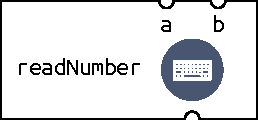
\includegraphics[scale=0.9]{../illustrations/function-readNumber.pdf}
\end{center}
Εικόνα: Η συνάρτηση \pyinline{readNumber} είναι ένα ανεξάρτητο τμήμα κώδικα, ένα αυτόνομο ``εξάρτημα'' που επιτελεί μια συγκεκριμένη λειτουργία.}
\begin{pynew}
def readNumber(a,b):
    print("Μάντεψε τον αριθμό.")
    print("Δοκίμασε ανάμεσα στο", a, "και το", b)
    c = int(input())    
    print("Έδωσες τον αριθμό", c)
    return c
\end{pynew}

Με τον τρόπο αυτό \emph{ορίζεται} η συνάρτηση \pyinline{readNumber}, η οποία λειτουργεί ως εξής: Δέχεται δύο παραμέτρους, δύο τιμές που τις ονομάζει \pyinline{a} και \pyinline{b} για να μπορεί να αναφέρεται σε αυτές. Προτρέπει το χρήστη να πληκτρολογήσει έναν αριθμό μεταξύ των \pyinline{a} και \pyinline{b} και \emph{επιστρέφει} με την εντολή \pyinline{return} την ακέραια τιμή που πληκτρολογεί ο χρήστης.

\begin{note}
Οι μεταβλητές \pyinline{a}, \pyinline{b} και \pyinline{c} έχουν \emph{τοπική εμβέλεια}, δηλαδή δεν είναι ``ορατές'' από το υπόλοιπο πρόγραμμα. Δημιουργούνται εκ νέου κάθε φορά που εκτελείται η συνάρτηση \pyinline{readNumber} και μετά παύουν να υφίστανται.
\end{note}

Γιατί φτιάξαμε αυτό το μικρό ``εξάρτημα''; Πρώτον, για να το χρησιμοποιήσουμε στο πρόγραμμά μας. Δεύτερον, για να μπορέσουμε αργότερα να το αντικαταστήσουμε με παρόμοια εξαρτήματα που κάνουν την ίδια δουλειά (επιστρέφουν μια πιθανή τιμή για τον μυστικό αριθμό) με διαφορετικό τρόπο.
\end{step}

\begin{step}
Κατασκευάσαμε ένα ``εξάρτημα'' που ονομάζεται \pyinline{readNumber} και επιτελεί μια συγκεκριμένη λειτουργία, ωστόσο δεν το έχουμε ακόμα \emph{χρησιμοποιήσει}.

\emph{Εντοπίστε} στο πρόγραμμά σας τις παρακάτω εντολές:

\begin{pyplain}
    print("Μάντεψε τον αριθμό.")
    print("Δοκίμασε ανάμεσα στο", low, "και το", high)
    number = int(input())    
    print("Έδωσες τον αριθμό", number)
\end{pyplain}

\emph{Διαγράψτε} τις και \emph{αντικαταστήστε} με την παρακάτω γραμμή:

\begin{pynew}
    number = readNumber(low, high)
\end{pynew}

Κατά την εκτέλεση του προγράμματος, αυτή η γραμμή θα \emph{καλέσει} την \pyinline{readNumber}, θα ενεργοποιήσει την εκτέλεση των εντολών της, παρέχοντας ως παραμέτρους τις τιμές των \pyinline{low} και \pyinline{high}. Την τιμή που επιστρέφεται από την συνάρτηση την ονομάζουμε \pyinline{number}.

Εκτελέστε το πρόγραμμα. Παρατηρείτε κάποια διαφορά στον τρόπο που λειτουργεί;

\begin{answer}
Όχι. Ως χρήστες δεν αντιλαμβανόμαστε καμία απολύτως διαφορά στα μηνύματα που βλέπουμε και στον τρόπο που αλληλεπιδρούμε με το πρόγραμμα. Ως προγραμματιστές όμως, παρατηρούμε ότι το κύριο πρόγραμμα είναι συντομότερο και φαίνεται απλούστερο στην κατανόηση της λειτουργίας του. 
\end{answer}
\end{step}

\begin{step}
\label{step:readNumber-call}
\emph{Προσθέστε} στην αρχή του προγράμματός σας τον κώδικα που ακολουθεί. \emph{Συμπληρώστε} κατάλληλα τις γραμμές που συνοδεύονται από σχόλιο, έτσι ώστε η συνάρτηση \pyinline{randNumber} που ορίζεται εδώ \emph{να επιστρέφει έναν τυχαίο αριθμό} ανάμεσα στα \pyinline{a} και \pyinline{b}.

\begin{pynew}
import time
def randNumber(a,b):
    print("Μάντεψε τον αριθμό.")
    print("Δοκίμασε ανάμεσα στο", a, "και το", b)
    c = |\textrm{\textit{επιλογή τυχαίου αριθμού}}|             # συμπληρώστε
    print("Το πρόγραμμα επιλέγει", c)
    time.sleep(3)
    return |\textrm{\textit{επιστροφή τιμής}}|                # συμπληρώστε
\end{pynew}

\begin{answer}
Το τμήμα κώδικα θα συμπληρωθεί όπως παρακάτω:

\begin{pyplain}
import time
def randNumber(a,b):
    print("Μάντεψε τον αριθμό.")
    print("Δοκίμασε ανάμεσα στο", a, "και το", b)
    c = |\pyhighlight{random.randint(a,b)}|
    print("Το πρόγραμμα επιλέγει", c)
    time.sleep(3)
    return |\pyhighlight{c}|
\end{pyplain}
\end{answer}

Στο κύριο πρόγραμμα, εντοπίστε την εντολή με την οποία η μεταβλητή \pyinline{number} παίρνει τιμή από την συνάρτηση \pyinline{readNumber} και \emph{προσθέστε} μπροστά από την εντολή το σύμβολο \#. Αυτό έχει σαν αποτέλεσμα η εντολή αυτή να θεωρείται \emph{σχόλιο} και να αγνοείται κατά την εκτέλεση του προγράμματος.

\begin{note}
Είναι συνηθισμένο να ``σχολιάζουμε'' μια εντολή όταν θέλουμε να παρακαμφθεί, χωρίς όμως να την αφαιρέσουμε πλήρως από το πρόγραμμα. Έτσι μπορούμε να την επαναφέρουμε αργότερα, αν αυτό είναι απαραίτητο.
\end{note}

Στο ίδιο σημείο, \emph{προσθέστε} μια εντολή με την οποία η μεταβλητή \pyinline{number} θα παίρνει τιμή από την συνάρτηση \pyinline{randNumber}, με παραμέτρους τις τιμές των \pyinline{low} και \pyinline{high}. Αν δυσκολευτείτε, ανατρέξτε στο βήμα~\ref{step:readNumber-call}, όπου γίνεται κάτι ανάλογο.

\begin{answer}
Η εντολή που θα προσθέσουμε στο πρόγραμμα (με την προηγούμενη εντολή σχολιασμένη) είναι:

\clearpage
% [comment] Λόγω τεχνικού προβλήματος με το minted (το # είναι escape character} δεν μπορεί να μπει το σχόλιο σε pyhighlight. Μικρό το κακό.
\begin{pyplain}
# number = readNumber(low,high)
\end{pyplain}
\begin{pynew}
number = randNumber(low,high)
\end{pynew}
\end{answer}

Ουσιαστικά, εκεί που το πρόγραμμα χρησιμοποιούσε τη \pyinline{readNumber} για να αποκτηθεί μια πιθανή τιμή για τον μυστικό αριθμό, τώρα αυτή αντικαταστάθηκε από την \pyinline{randNumber}.

Χρησιμοποιείται πουθενά στο πρόγραμμα η \pyinline{input}, για να παρέχει οποιαδήποτε είσοδο ο χρήστης; Αν όχι, ποιος θα επιλέγει τώρα αριθμούς, προσπαθώντας να μαντέψει τον τυχαίο αριθμό;

\begin{answer}
Όχι, ο χρήστης δεν δίνει πλέον τιμές. Στην ουσία το ρόλο του παίκτη τον έχει αναλάβει το ίδιο το πρόγραμμα, το οποίο παράγει τυχαίους αριθμούς προσπαθώντας να μαντέψει το μυστικό αριθμό.
\end{answer}

Εκτελέστε το πρόγραμμα. Τι αλλαγή επιφέρει η χρήση της συνάρτησης \pyinline{randNumber}, αντί για τη \pyinline{readNumber};

\begin{answer}
Ο ρόλος του παίκτη ανατίθεται πλέον στο ίδιο το πρόγραμμα.
\end{answer}
\end{step}

\begin{step}
Όταν ξεκινά το πρόγραμμα και γνωρίζετε ότι ο μυστικός αριθμός βρίσκεται κάπου ανάμεσα στο \pyinline{1} και το \pyinline{32}, ποια τιμή σας φαίνεται προτιμότερο να επιλέξετε;

\begin{answer}
Η καλύτερη τιμή είναι το \pyinline{16}. Χωρίζοντας το διάστημα των αριθμών στη μέση θα ``διώξουμε'' με μια κίνηση τους μισούς αριθμούς.
\end{answer}

Αν γνωρίζετε ότι ο μυστικός αριθμός βρίσκεται κάπου ανάμεσα στο \pyinline{13} και το \pyinline{23}, ποια τιμή σας φαίνεται προτιμότερο να επιλέξετε;

\begin{answer}
Ακολουθώντας την ίδια λογική θα επιλέξουμε την τιμή \pyinline{18}.
\end{answer}

Αν γνωρίζετε ότι ο μυστικός αριθμός βρίσκεται κάπου ανάμεσα στο \pyinline{low} και το \pyinline{high}, ποια τιμή σας φαίνεται προτιμότερο να επιλέξετε και γιατί;

\begin{answer}
Γενικεύοντας το σκεπτικό των προηγούμενων βημάτων θα επιλέγαμε την τιμή που βρίσκεται στη μέση του διαστήματος (\pyinline{low}, \pyinline{high}), υπολογίζοντας την τιμή της παράστασης \pyinline{(low + high)} // 2.
\end{answer}

\end{step}

\begin{step}
Κατασκευάστε μια συνάρτηση \pyinline{midNumber}. Η συνάρτηση θα δέχεται σαν παραμέτρους δύο τιμές, που θ' αντιστοιχούν στα όρια του διαστήματος μέσα στο οποίο γνωρίζουμε ότι βρίσκεται ο μυστικός αριθμός, και θα επιστρέφει την τιμή που βρίσκεται%
\marginnote[3pt]{Ο μυστικός αριθμός είναι ακέραιος, άρα η τιμή που επιλέγει η \pyinline{midNumber} πρέπει να είναι επίσης ακέραια. Φροντίστε να χρησιμοποιήσετε τον τελεστή \pyinline{//} της \emph{ακέραιας} διαίρεσης για τον υπολογισμό του μέσου του διαστήματος.}
\emph{στο μέσο αυτού του διαστήματος}.

\begin{note}
Χρησιμοποιήστε ως πρότυπα τις \pyinline{readNumber} και \pyinline{randNumber}.
\end{note}

\begin{answer}
Η συνάρτηση \pyinline{midNumber} θα είναι όπως παρακάτω:

\begin{pynew}
def midNumber(a,b):
    print("Μάντεψε τον αριθμό:", a , "-", b)
    num = (a + b) // 2
    print("Ο υπολογιστής επιλέγει:", num)
    return num
\end{pynew}
\end{answer}

\clearpage
Στο κύριο πρόγραμμα, εντοπίστε την εντολή με την οποία η μεταβλητή \pyinline{number} παίρνει τιμή από την συνάρτηση \pyinline{randNumber} και \emph{προσθέστε} μπροστά από την εντολή το σύμβολο \#.

Στο ίδιο σημείο, \emph{προσθέστε} μια εντολή με την οποία η μεταβλητή \pyinline{number} θα παίρνει τιμή από την συνάρτηση \pyinline{midNumber}, με παραμέτρους τις τιμές των \pyinline{low} και \pyinline{high}.

\begin{answer}
Η εντολή που θα προσθέσουμε για να καλέσουμε την \pyinline{midNumber} είναι: 

\begin{pynew}
number = midNumber(low,high)
\end{pynew}
\end{answer}
\end{step}

Εκτελέστε το πρόγραμμα μερικές φορές. Καταφέρνει να εντοπίσει τον μυστικό αριθμό;

\begin{answer}
Ναι, το πρόγραμμα κατορθώνει κάποιες φορές να μαντέψει το μυστικό αριθμό. Τις υπόλοιπες πέφτει πολύ κοντά! Αν δοκιμάσουμε να του δώσουμε μια ακόμα προσπάθεια, δηλαδή \pyinline{5} συνολικά τότε θα καταφέρνει να τον μαντεύει σε όλες τις περιπτώσεις.
\end{answer}
\end{document}
